
\documentclass{beamer}		% This tells LaTeX the document will be a "beamer" presentation

\mode<presentation>
{
  \usetheme{Madrid}      % or try Darmstadt, Madrid, Warsaw, ...
  \usecolortheme{default} % or try albatross, beaver, crane, ...
  \usefonttheme{serif}  % or try serif, structurebold, ...
  \setbeamertemplate{navigation symbols}{}
  \setbeamertemplate{caption}[numbered]
} 

\usepackage{amsmath}
\usepackage{amssymb}
\usepackage{amsfonts}
\usepackage{bm}
\usepackage{graphicx}

\usepackage[backend=bibtex,sorting=none]{biblatex}
\addbibresource{references.bib}
\setbeamerfont{footnote}{size=\tiny}
\setbeamertemplate{bibliography item}[text]
\newcommand{\dd}{\mathrm{d}}

\title[Optimal transport mapping via input convex neural networks]{Optimal transport mapping via input convex neural networks}	% Insert your title.  Depending on the theme you choose above, a "short title" might be useful, as it will appear on the footer of each slide.

\author[Shen Yuan]{Ashok Vardhan Makkuva \quad Amirhossein Taghvaei \quad  Jason D. Lee  \quad Sewoong Oh} % Insert your name

% \institute[UoE]{University of Edinburgh} % Self-explanatory



\begin{document} 	% Let's begin

% Presentations come in slide frames.  You have to tell LaTeX when to start a frame, and when to end the frame.  The most common error beginners make with beamer is forgetting the \end{frame} command.	

\newcommand{\light}[1]{\textcolor{gray}{#1}}

\begin{frame}	

\titlepage	% Prints a title page populated with the information given in the preamble
	
\end{frame}	




\begin{frame}[noframenumbering]

\begin{itemize}

    \begin{LARGE}
    
    \item Introduction
    
    \item \light{Formulation of 2-Wasserstein distance}
    
    \item \light{Minimax optimization over ICNNs}
    
    \item \light{Expriments}

    \end{LARGE}
    
\end{itemize}
	
\end{frame}






% \begin{frame}{Background}
% $\bm{Network\ Formation\ Model}$
% \begin{figure}
% 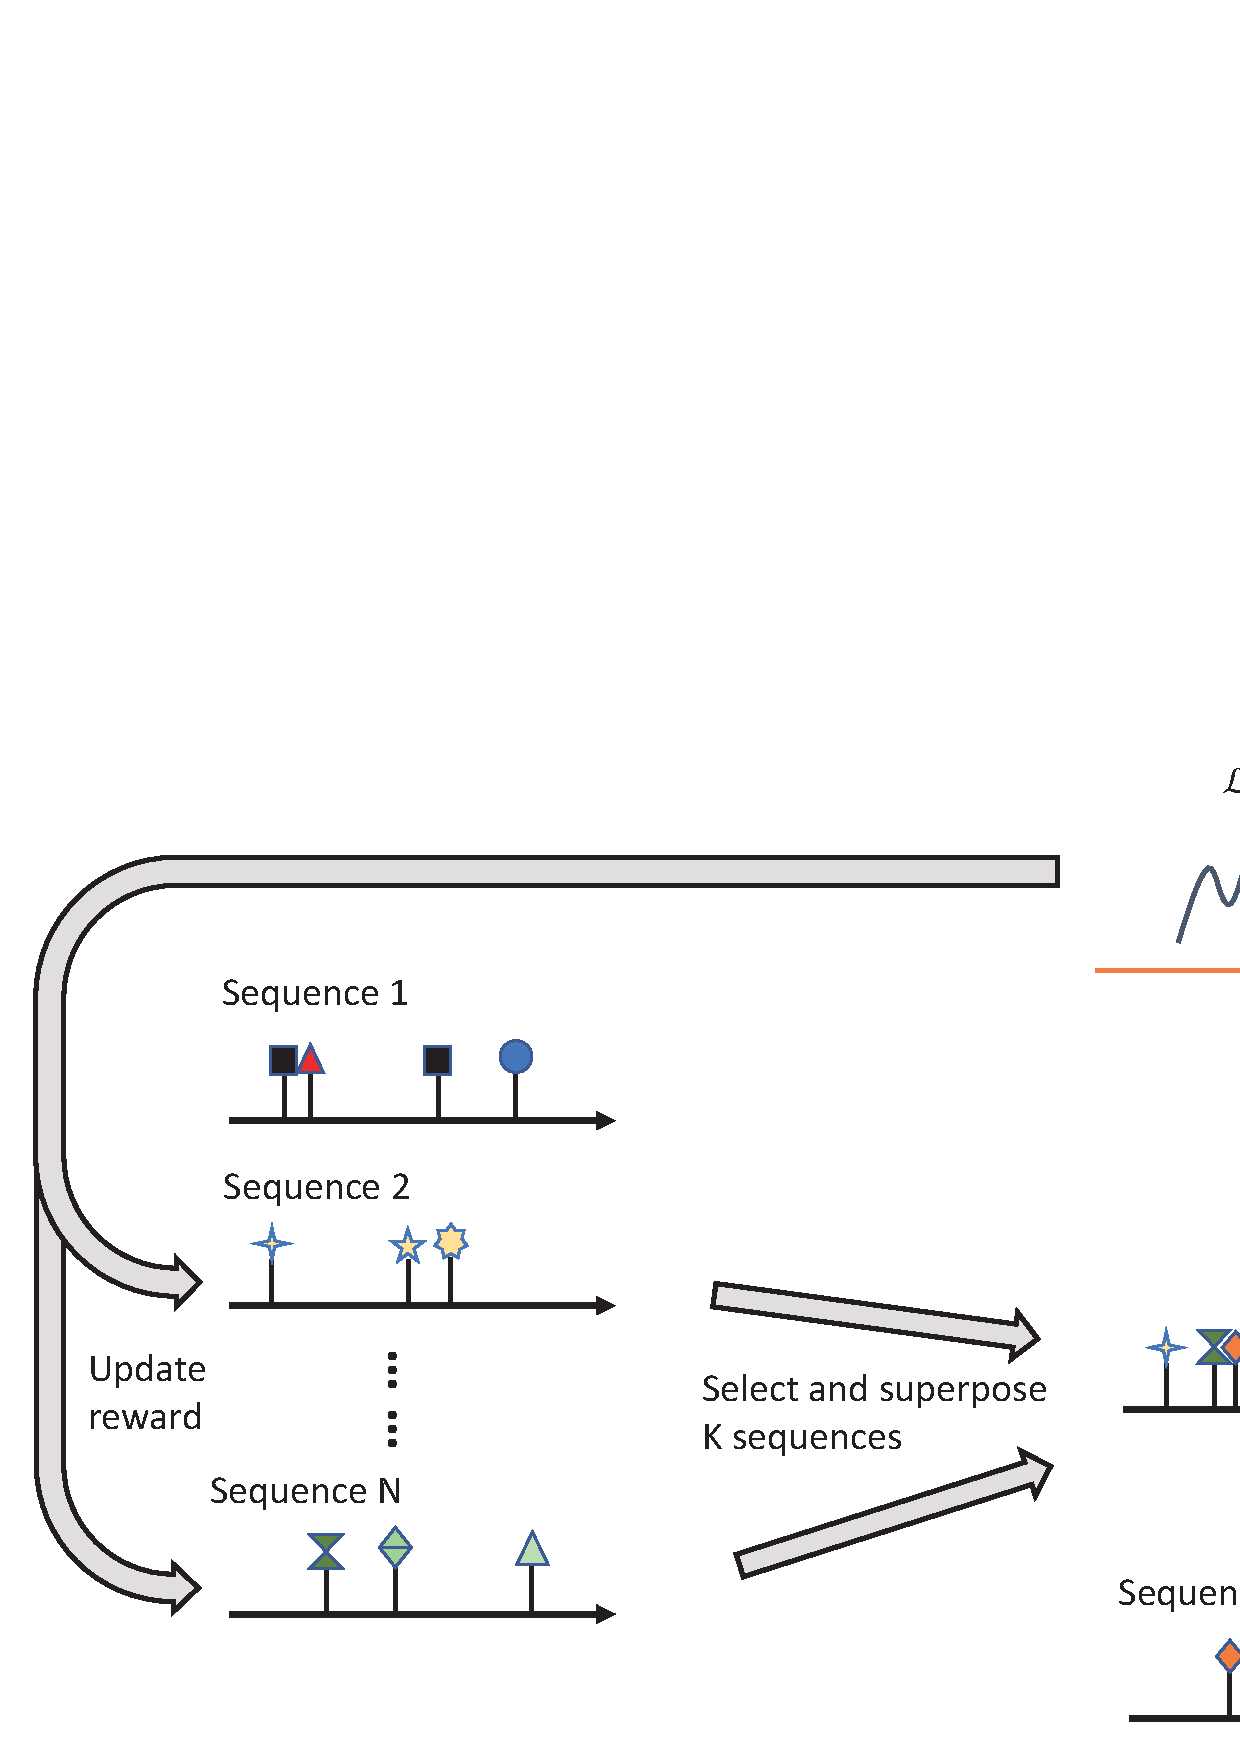
\includegraphics[height=6cm]{figure1.jpg}
% \end{figure}
% \end{frame}



\begin{frame}{Notation}
    \begin{itemize}
        \item $\mathcal{P(X)}$, the set of probability measures
        on a Polish space $\mathcal{X}$. $P,Q\in\mathcal{P(X)}$
        \item $\mathcal{B(X)}$, the Borel subsets of $\mathcal{X}$
        \item $T:\mathcal{X} \to \mathcal{Y}$, the measurable map, $(T\#Q)(A)=Q(T^{-1}(A)), \forall A\in \mathcal{B(Y)}$
        \item $L^1(P):=\{f\ is\ measurable\ \& \int f\ \dd P < \infty \}$.
        \item $CVX(P)$, the set of all convex functions in $L^1(P)$.
    \end{itemize}    
\end{frame}



% \begin{frame}{Introduction}

% \begin{eqnarray*}
% \begin{aligned}
% W_2^2 (P, Q)
% \end{aligned}    
% \end{eqnarray*}

% \begin{eqnarray*}\label{eq:minimmax}
% \begin{aligned}
% W_2^2 (P, Q) = \sup_{f} \ \inf_{g} \  \mathcal{V}_{P,Q} (f,g) + C_{P,Q}
% \end{aligned}    
% \end{eqnarray*}

% \begin{figure}[t]
% \centerline{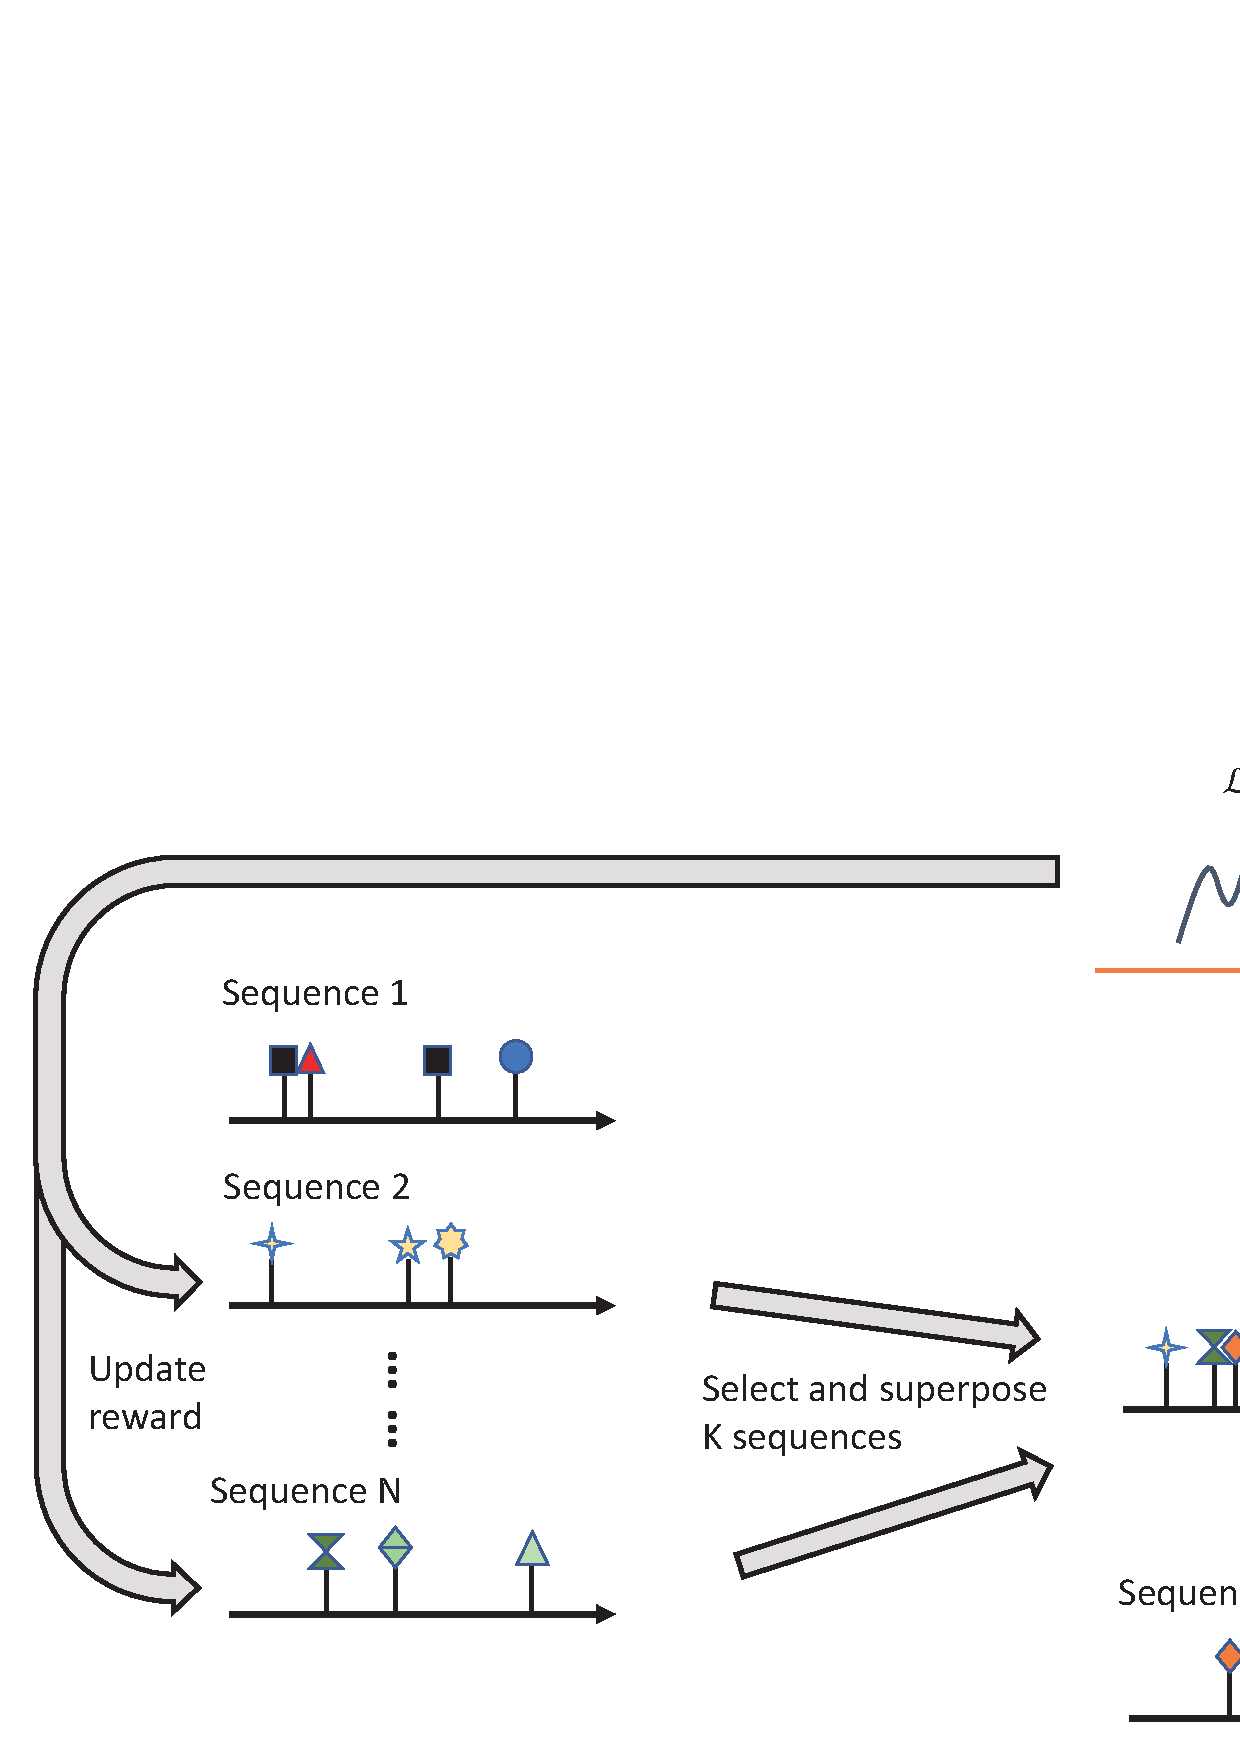
\includegraphics[width=0.5\linewidth]{figure1.pdf}}
% \vspace{-10pt}

% \label{fig1}
% \end{figure}

% \end{frame}


\begin{frame}{Introduction}


\begin{figure}[t]
\centerline{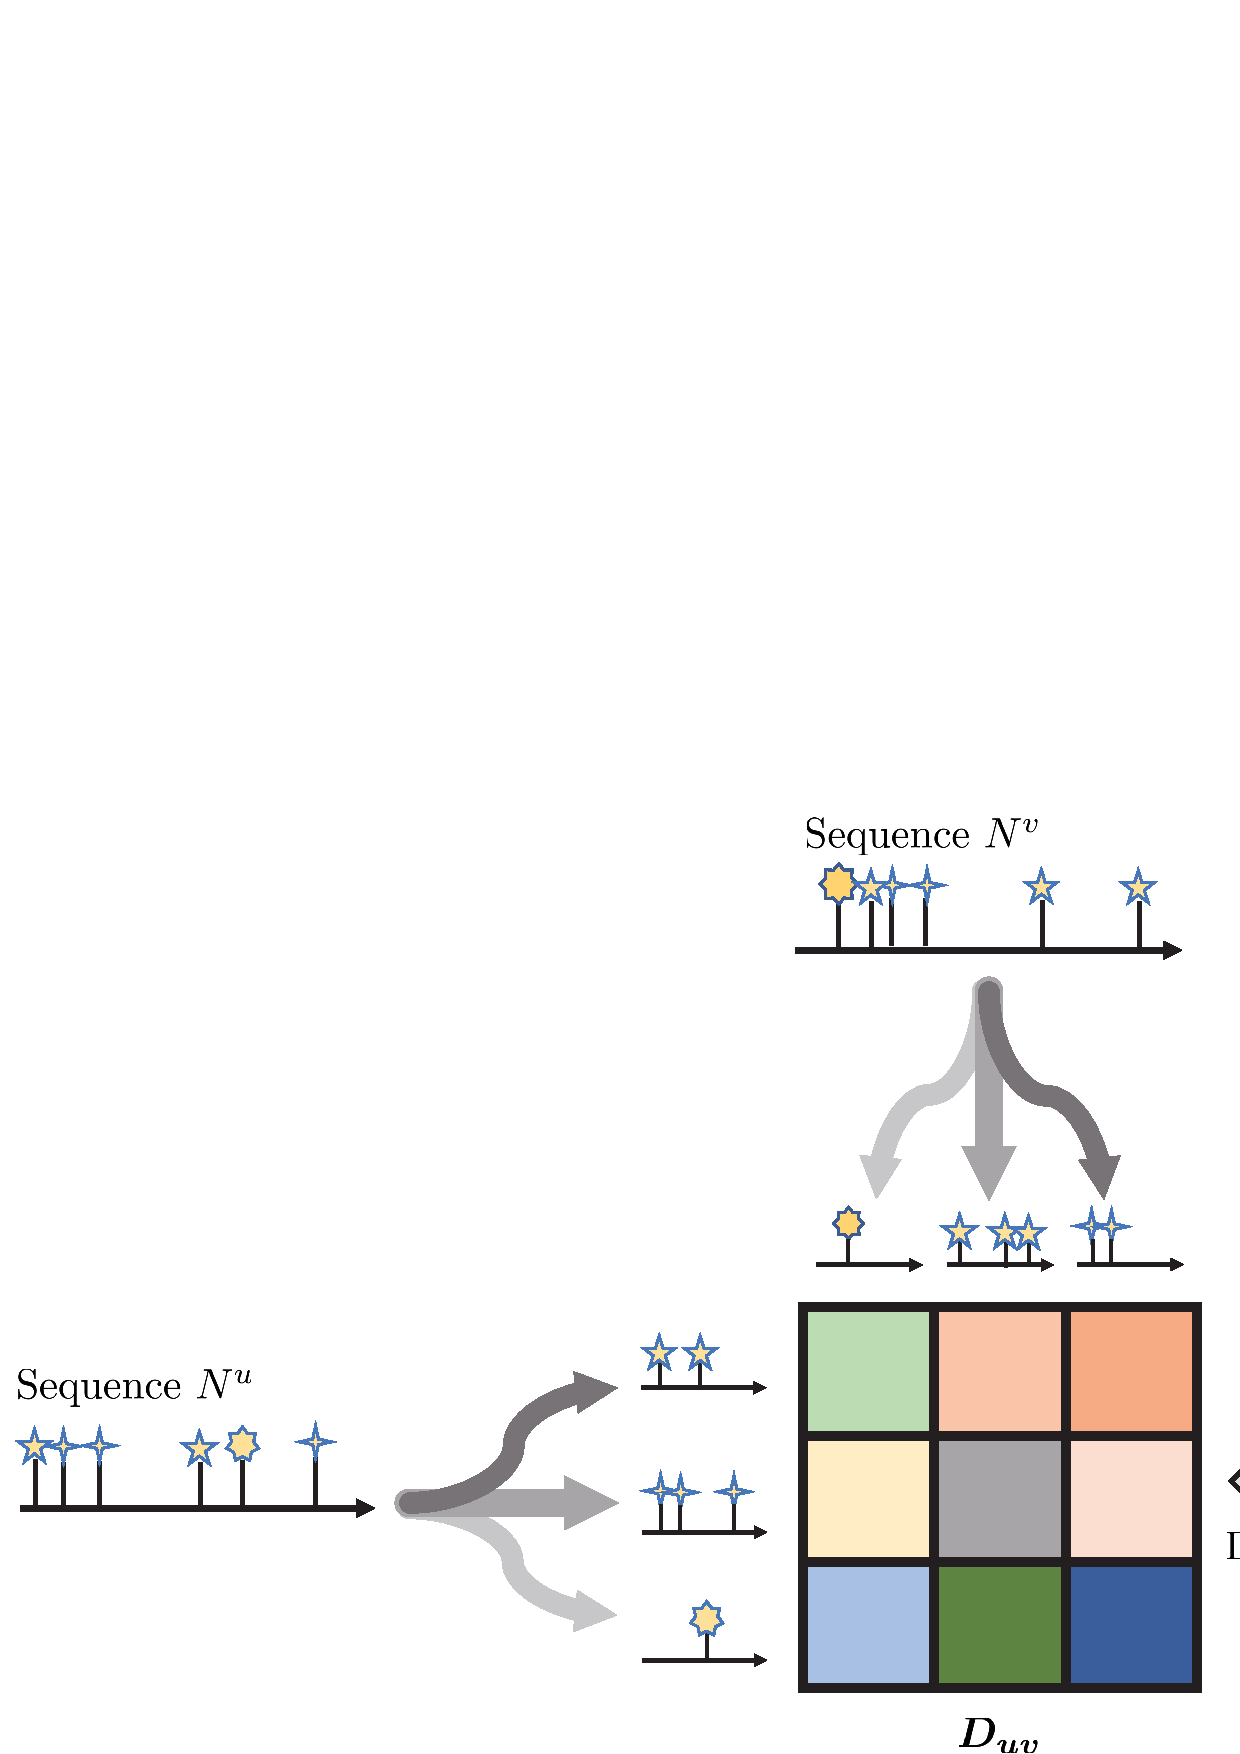
\includegraphics[width=0.6\linewidth]{figure2.pdf}}
\vspace{-10pt}

\label{fig1}
\end{figure}


\end{frame}











\begin{frame}[noframenumbering]

    \begin{itemize}
    
        \begin{LARGE}
        
        \item \light{Introduction}
        
        \item Formulation of 2-Wasserstein distance
        
        \item \light{Minimax optimization over ICNNs}
        
        \item \light{Expriments}
    
        \end{LARGE}
        
    \end{itemize}
        
    \end{frame}







\begin{frame}{Formulation of 2-Wasserstein distance}

This part builds on the work in \footfullcite{taghvaei20192}, which restricts the optimization problem to the variants of convex functions and leverages the input-convex neural networks to approximate 2-Wasserstein distance.

    
\end{frame}











\begin{frame}{Formulation of 2-Wasserstein distance}

\begin{eqnarray}\label{eq:W2origin}
\begin{aligned}
W_2^2 (P, Q) = \inf_{\pi \in \prod (P,Q)} \frac{1}{2} \mathbb{E}_{(X,Y) \sim \pi} \left\| X - Y \right\|^2
\end{aligned}    
\end{eqnarray}

where $\prod (P,Q)$ denotes the set of all joint probability distributions whose first and second marginals are P and Q.

\pause

\begin{eqnarray}\label{eq:W2dual}
\begin{aligned}
W_2^2 (P, Q) = \sup_{(f,g) \in \Phi_c} \mathbb{E}_P [f(X)] + \mathbb{E}_Q [ g(Y) ]
\end{aligned}    
\end{eqnarray}

where $\Phi_c := \{ (f,g) \in L^1(P) \times L^1(Q): f(x)+g(y) \leq \frac{1}{2} \left\|x-y \right\|_2^2, \forall (x,y) \dd P \otimes \dd Q \}$


    
\end{frame}









\begin{frame}{Formulation of 2-Wasserstein distance}

\begin{eqnarray*}
\begin{aligned}
    & f(x)+g(y) \leq \frac{1}{2} \left\|x-y \right\|_2^2 \\
    \pause
    \Longleftrightarrow\ &\left[\frac{1}{2} \left\| x\right\|_2^2-f(x) \right] + \left[\frac{1}{2} \left\| y\right\|_2^2-g(y) \right] \ge \left \langle x,y \right \rangle\\
    \pause
    \Longleftrightarrow\ & f(x) + g(y) \ge \left \langle x,y \right \rangle
\end{aligned}    
\end{eqnarray*}

Reparametrizing $\frac{1}{2} \left\| \cdot \right\|_2^2-f(\cdot)$ and $\frac{1}{2} \left\| \cdot \right\|_2^2-g(\cdot)$ by $f$ and $g$,
    
\end{frame}










\begin{frame}{Formulation of 2-Wasserstein distance}

\begin{eqnarray}\label{eq:W2dual2}
\begin{aligned}
W_2^2 (P, Q) = \sup_{(f,g) \in \tilde{\Phi}_c} \mathbb{E}_P \left[\frac{1}{2} \left\| X\right\|_2^2-f(X) \right] + \mathbb{E}_Q \left[ \frac{1}{2} \left\| Y\right\|_2^2-g(Y) \right]
\end{aligned}    
\end{eqnarray}

where $\tilde{\Phi}_c := \{ (f,g) \in L^1(P) \times L^1(Q): f(x)+g(y) \ge \left \langle x,y \right \rangle, \forall (x,y) \dd P \otimes \dd Q \}$

\pause

\begin{eqnarray*}
\begin{aligned}
W_2^2 (P, Q)=\frac{1}{2} \mathbb{E}[\left\|X \right\|_2^2 + \left\|Y \right\|_2^2] + \sup_{(f,g) \in \tilde{\Phi}_c} \left[- \mathbb{E}_P[f(X)] - \mathbb{E}_Q[g(Y)] \right]
\end{aligned}    
\end{eqnarray*}


    
\end{frame}







\begin{frame}{Formulation of 2-Wasserstein distance}

\textbf{Theroem 2.9 (Existence of an optimal pair of convex conjugate functions) \footfullcite{villani2003topics} } Let $P, Q$ be two probability measures on $\mathbb{R}^d$, with finite second order moments. There exists a pair $(f, f^*)$ of lower semi-continuous proper conjugate convex functions on $\mathbb{R}^d$, then we can get

\begin{eqnarray}
\begin{aligned}
W_2^2 (P, Q) = C_{P,Q} + \sup_{f \in CVX(P)} \left[ - \mathbb{E}_P[f(X)] - \mathbb{E}_Q[f^*(Y)] \right]
\end{aligned}    
\end{eqnarray}

where $C_{P,Q} = \frac{1}{2} \mathbb{E}[\left\|X \right\|_2^2 + \left\|Y \right\|_2^2] $, and $f^*(y)=\sup_x \left \langle x,y \right \rangle - f(x)$ is the convex conjugate of $f(\cdot)$.

\end{frame}













\begin{frame}[noframenumbering]

\begin{itemize}

    \begin{LARGE}
    
    \item \light{Introduction}
    
    \item \light{Formulation of 2-Wasserstein distance}
    
    \item Minimax optimization over ICNNs
    
    \item \light{Expriments}

    \end{LARGE}
    
\end{itemize}
    
\end{frame}









\begin{frame}{Minimax formulation}

\begin{eqnarray*}
\begin{aligned}
W_2^2 (P, Q) = C_{P,Q} + \sup_{f \in CVX(P)} \left[- \mathbb{E}_P[f(X)] - \mathbb{E}_Q[f^*(Y)] \right]
\end{aligned}    
\end{eqnarray*}

\pause

Using a minimax formulation, 

\begin{eqnarray}\label{eq:minimmax}
\begin{aligned}
W_2^2 (P, Q) = C_{P,Q} + \sup_{f\in CVX(P)} \ \inf_{g \in CVX(Q)} \  \mathcal{V}_{P,Q} (f,g)
\end{aligned}    
\end{eqnarray}

where

\begin{eqnarray}\label{eq:minimmax}
\begin{aligned}
\mathcal{V}_{P,Q}=-\mathbb{E}_P[f(X)]-\mathbb{E}_Q[\left \langle Y,\nabla g(Y) \right \rangle - f(\nabla g(Y))]
\end{aligned}    
\end{eqnarray}

\end{frame}








\begin{frame}{Minimax formulation}

\begin{eqnarray*}
\begin{aligned}
f^*(Y) \ &\ge \ \left \langle Y,\nabla g(Y) \right \rangle - f(\nabla g(Y))
\\
\pause
\\
\mathbb{E}_Q[f^*(Y)] \ &\ge \ \mathbb{E}_Q[\left \langle Y,\nabla g(Y) \right \rangle - f(\nabla g(Y))] 
\\
\pause
\\
- \mathbb{E}_Q[f^*(Y)] \ &\leq \ -\mathbb{E}_Q[\left \langle Y,\nabla g(Y) \right \rangle - f(\nabla g(Y))] 
\\
\pause
\\
- \mathbb{E}_P[f(X)] - \mathbb{E}_Q[f^*(Y)] \ &\leq \ -\mathbb{E}_P[f(X)]-\mathbb{E}_Q[\left \langle Y,\nabla g(Y) \right \rangle - f(\nabla g(Y))]
\\
\pause
\\
- \mathbb{E}_P[f(X)] - \mathbb{E}_Q[f^*(Y)] \ &= \  \inf_{g \in CVX(Q)} \  \mathcal{V}_{P,Q} (f,g)
\end{aligned}    
\end{eqnarray*}



\end{frame}




\begin{frame}{Minimax formulation}

\begin{eqnarray*}
\begin{aligned}
\nabla g(y) &= \nabla (\frac{1}{2} \left\|y \right\|_2^2 - g_{o}(y)) \\
&= y - \nabla g_{o}(y)
\end{aligned}    
\end{eqnarray*}

Suppose $T$ is the optimal transport map, then $\nabla g_{o}(y) =$ $ \nabla_y \frac{1}{2}  \left\| x - y \right\|_2^2 = y - x$, plugging it into above, we can get $\nabla g(y) = x$.

~\\
By the defination of convex conjugate, $f^*(y)=\sup_x \left \langle x,y \right \rangle - f(x)$, then we can get $f^*(y) \ = \ \left \langle y,\nabla g(y) \right \rangle - f(\nabla g(y))$

\end{frame}





% \begin{frame}{Minimax formulation}

% \begin{eqnarray*}
% \begin{aligned}
% W_2^2 (P, Q) =\sup_{f\in CVX(P)} \ \inf_{g \in CVX(Q)} \  \mathcal{V}_{P,Q} (f,g) + C_{P,Q}
% \end{aligned}    
% \end{eqnarray*}

% For any convex function $f$, the function $g \in L^1(Q)$ that achieves the infimum is convex and equals $f^*$,

% \begin{eqnarray}
% \begin{aligned}
% W_2^2 (P, Q) =\sup_{f\in CVX(P)} \ \inf_{g \in L^1(Q)} \  \mathcal{V}_{P,Q} (f,g) + C_{P,Q}
% \end{aligned}    
% \end{eqnarray}

% \end{frame}








\begin{frame}{ICNN}

\begin{figure}
\includegraphics[height=3cm]{figure3.png}
\caption{The input convex neural network (ICNN) architecture}
\end{figure}

\begin{eqnarray}
\begin{aligned}
z_{l+1}=\sigma_l(W_lz_l+A_lx+b_l),\ f(x;\theta)=z_L
\end{aligned}    
\end{eqnarray}

where $\{W_l\}$, $\{A_l\}$ are weight matrices, and $\{b_l\}$ are the bias terms, and $\theta = (\{W_l\}, \{A_l\}, \{b_l\})$.

\end{frame}






\begin{frame}{ICNN}


\begin{eqnarray}
\begin{aligned}
z_{l+1}=\sigma_l(W_lz_l+A_lx+b_l),\ f(x;\theta)=z_L
\end{aligned}    
\end{eqnarray}

To ensure that $f(x;\theta)$ is convex, 

\begin{itemize}
    \item all entries of the weights $W_l$ are non-negative
    \item activation function $\sigma_0$ is convex
    \item $\sigma_l$ is convex and non-decreasing, for $l = 1,\ldots,L-1$.
\end{itemize}

\end{frame}







\begin{frame}{Minimax optimization over ICNNs}


\begin{eqnarray}
\begin{aligned}
\max_{\theta_f} \min_{\theta_g} J(\theta_f, \theta_g) + R(\theta)
\end{aligned}    
\end{eqnarray}
where $R(\cdot)$ denotes the regularization term, and $J(\theta_f, \theta_g)=\frac{1}{M} \sum_{i=1}^{M} - f(X_i) - \left \langle Y_i, \nabla g(Y_i)\right \rangle + f(\nabla g(Y_i)) $ corresponding to 

\begin{eqnarray*}
\begin{aligned}
\mathcal{V}_{P,Q}=-\mathbb{E}_P[f(X)]-\mathbb{E}_Q \left[\left \langle Y,\nabla g(Y) \right \rangle - f(\nabla g(Y)) \right]
\end{aligned}    
\end{eqnarray*}




\end{frame}







\begin{frame}{Minimax optimization over ICNNs}


\begin{figure}
\includegraphics[height=5.5cm]{figure4.png}
\end{figure}


\end{frame}
    








\begin{frame}[noframenumbering]

\begin{itemize}

    \begin{LARGE}
    
    \item \light{Introduction}
    
    \item \light{Formulation of 2-Wasserstein distance}
    
    \item \light{Minimax optimization over ICNNs}
    
    \item Expriments

    \end{LARGE}
    
\end{itemize}
    
\end{frame}




\begin{frame}{Minimax optimization over ICNNs}
\begin{figure}
\includegraphics[height=5cm]{figure5.png}
\caption{The transport maps learned by various approaches on ‘Checker board’ and ‘mixture of eight Gaussians’ datasets.}
\end{figure}
\end{frame}


\end{document}	% Done!

